% Options for packages loaded elsewhere
% Options for packages loaded elsewhere
\PassOptionsToPackage{unicode}{hyperref}
\PassOptionsToPackage{hyphens}{url}
\PassOptionsToPackage{dvipsnames,svgnames,x11names}{xcolor}
%
\documentclass[
  11pt,
]{article}
\usepackage{xcolor}
\usepackage[margin=1in]{geometry}
\usepackage{amsmath,amssymb}
\setcounter{secnumdepth}{5}
\usepackage{iftex}
\ifPDFTeX
  \usepackage[T1]{fontenc}
  \usepackage[utf8]{inputenc}
  \usepackage{textcomp} % provide euro and other symbols
\else % if luatex or xetex
  \usepackage{unicode-math} % this also loads fontspec
  \defaultfontfeatures{Scale=MatchLowercase}
  \defaultfontfeatures[\rmfamily]{Ligatures=TeX,Scale=1}
\fi
\usepackage{lmodern}
\ifPDFTeX\else
  % xetex/luatex font selection
\fi
% Use upquote if available, for straight quotes in verbatim environments
\IfFileExists{upquote.sty}{\usepackage{upquote}}{}
\IfFileExists{microtype.sty}{% use microtype if available
  \usepackage[]{microtype}
  \UseMicrotypeSet[protrusion]{basicmath} % disable protrusion for tt fonts
}{}
\makeatletter
\@ifundefined{KOMAClassName}{% if non-KOMA class
  \IfFileExists{parskip.sty}{%
    \usepackage{parskip}
  }{% else
    \setlength{\parindent}{0pt}
    \setlength{\parskip}{6pt plus 2pt minus 1pt}}
}{% if KOMA class
  \KOMAoptions{parskip=half}}
\makeatother
% Make \paragraph and \subparagraph free-standing
\makeatletter
\ifx\paragraph\undefined\else
  \let\oldparagraph\paragraph
  \renewcommand{\paragraph}{
    \@ifstar
      \xxxParagraphStar
      \xxxParagraphNoStar
  }
  \newcommand{\xxxParagraphStar}[1]{\oldparagraph*{#1}\mbox{}}
  \newcommand{\xxxParagraphNoStar}[1]{\oldparagraph{#1}\mbox{}}
\fi
\ifx\subparagraph\undefined\else
  \let\oldsubparagraph\subparagraph
  \renewcommand{\subparagraph}{
    \@ifstar
      \xxxSubParagraphStar
      \xxxSubParagraphNoStar
  }
  \newcommand{\xxxSubParagraphStar}[1]{\oldsubparagraph*{#1}\mbox{}}
  \newcommand{\xxxSubParagraphNoStar}[1]{\oldsubparagraph{#1}\mbox{}}
\fi
\makeatother


\usepackage{longtable,booktabs,array}
\usepackage{calc} % for calculating minipage widths
% Correct order of tables after \paragraph or \subparagraph
\usepackage{etoolbox}
\makeatletter
\patchcmd\longtable{\par}{\if@noskipsec\mbox{}\fi\par}{}{}
\makeatother
% Allow footnotes in longtable head/foot
\IfFileExists{footnotehyper.sty}{\usepackage{footnotehyper}}{\usepackage{footnote}}
\makesavenoteenv{longtable}
\usepackage{graphicx}
\makeatletter
\newsavebox\pandoc@box
\newcommand*\pandocbounded[1]{% scales image to fit in text height/width
  \sbox\pandoc@box{#1}%
  \Gscale@div\@tempa{\textheight}{\dimexpr\ht\pandoc@box+\dp\pandoc@box\relax}%
  \Gscale@div\@tempb{\linewidth}{\wd\pandoc@box}%
  \ifdim\@tempb\p@<\@tempa\p@\let\@tempa\@tempb\fi% select the smaller of both
  \ifdim\@tempa\p@<\p@\scalebox{\@tempa}{\usebox\pandoc@box}%
  \else\usebox{\pandoc@box}%
  \fi%
}
% Set default figure placement to htbp
\def\fps@figure{htbp}
\makeatother





\setlength{\emergencystretch}{3em} % prevent overfull lines

\providecommand{\tightlist}{%
  \setlength{\itemsep}{0pt}\setlength{\parskip}{0pt}}



 


\usepackage{booktabs}
\usepackage{longtable}
\usepackage{array}
\usepackage{multirow}
\usepackage{wrapfig}
\usepackage{float}
\usepackage{colortbl}
\usepackage{pdflscape}
\usepackage{tabu}
\usepackage{threeparttable}
\usepackage{threeparttablex}
\usepackage[normalem]{ulem}
\usepackage{makecell}
\usepackage{xcolor}
\usepackage{booktabs}
\usepackage{longtable}
\usepackage{adjustbox}
\usepackage{float}
\makeatletter
\@ifpackageloaded{caption}{}{\usepackage{caption}}
\AtBeginDocument{%
\ifdefined\contentsname
  \renewcommand*\contentsname{Table of contents}
\else
  \newcommand\contentsname{Table of contents}
\fi
\ifdefined\listfigurename
  \renewcommand*\listfigurename{List of Figures}
\else
  \newcommand\listfigurename{List of Figures}
\fi
\ifdefined\listtablename
  \renewcommand*\listtablename{List of Tables}
\else
  \newcommand\listtablename{List of Tables}
\fi
\ifdefined\figurename
  \renewcommand*\figurename{Figure}
\else
  \newcommand\figurename{Figure}
\fi
\ifdefined\tablename
  \renewcommand*\tablename{Table}
\else
  \newcommand\tablename{Table}
\fi
}
\@ifpackageloaded{float}{}{\usepackage{float}}
\floatstyle{ruled}
\@ifundefined{c@chapter}{\newfloat{codelisting}{h}{lop}}{\newfloat{codelisting}{h}{lop}[chapter]}
\floatname{codelisting}{Listing}
\newcommand*\listoflistings{\listof{codelisting}{List of Listings}}
\makeatother
\makeatletter
\makeatother
\makeatletter
\@ifpackageloaded{caption}{}{\usepackage{caption}}
\@ifpackageloaded{subcaption}{}{\usepackage{subcaption}}
\makeatother
\usepackage{bookmark}
\IfFileExists{xurl.sty}{\usepackage{xurl}}{} % add URL line breaks if available
\urlstyle{same}
\hypersetup{
  pdftitle={Outer Sorting Baseline Simulation Memo},
  pdfauthor={Philly Evictions Project},
  colorlinks=true,
  linkcolor={blue},
  filecolor={Maroon},
  citecolor={Blue},
  urlcolor={Blue},
  pdfcreator={LaTeX via pandoc}}


\title{Outer Sorting Baseline Simulation Memo}
\author{Philly Evictions Project}
\date{2026-03-06}
\begin{document}
\maketitle

\renewcommand*\contentsname{Table of contents}
{
\hypersetup{linkcolor=}
\setcounter{tocdepth}{3}
\tableofcontents
}

\section{Overview}\label{overview}

This memo summarizes the baseline outer sorting simulation currently
implemented in \texttt{r/simulate-outer-sorting.R} and the associated
first-pass calibration setup in \texttt{r/calibrate-outer-sorting.R}.

The baseline normalization is:

\[
\bar\delta_b = s_b\delta_H + (1 - s_b)\delta_L,
\qquad
\log \bar f_b = a_F + b_{F\theta}\mathbf{1}\{\theta_b = B\} + b_{F\delta}\bar\delta_b,
\qquad
x_b \equiv \bar f_b,
\qquad
s_b^\star(\xi) = \Lambda(\xi + \Delta \alpha \bar f_b).
\]

The filing block now maps building composition into expected filings
through average tenant default risk rather than through a direct
reduced-form composition slope. The sorting signal is still the expected
filing rate, and the simulation iterates on expected maintenance,
complaint, and filing rates until the building composition vector is a
fixed point under the citywide mass constraint.

\section{Simulation Setup}\label{simulation-setup}

The baseline parameterization fixes the citywide high-risk share at
\(\mu = 0.30\), interpretable as a rough renter-poverty /
precarious-tenant share. The tenant default anchors are set to
\(\delta_L = 0.01\) and \(\delta_H = 0.10\), implying an average
anchored default probability of roughly 0.037.

The baseline filing block now uses average default risk,
\(\bar\delta_b = s_b\delta_H + (1-s_b)\delta_L\), so the anchored
tenant-side parameters are active inputs to the equilibrium. The
first-pass design calibrates the outer-layer parameters governing
sorting, tract-level bad-type dispersion, filing, complaints, and
maintenance. Simulated building units are now drawn by empirical
resampling from the observed PID-level average annual
\texttt{total\_units} distribution in \texttt{bldg\_panel\_blp} over
2011-2019, rather than from the old stylized unit bins.

\begin{table}
\tiny

\caption{Baseline outer sorting parameters}
\centering
\begin{tabular}[t]{llrll}
\toprule
block & parameter & value & status & note\\
\midrule
Tenant-side anchors & mu & 0.30 & Fixed & Citywide high-risk / precarious tenant share.\\
Tenant-side anchors & delta\_L & 0.01 & Fixed & Anchored low-risk default probability.\\
Tenant-side anchors & delta\_H & 0.10 & Fixed & Anchored high-risk default probability.\\
Built environment & p\_bad\_shape1 & 2.00 & Calibrated & Beta shape parameter for tract bad-type prevalence.\\
Built environment & p\_bad\_shape2 & 6.00 & Calibrated & Beta shape parameter for tract bad-type prevalence.\\
Sorting & Dalph & 6.00 & Calibrated & Sorting strength in the logistic update.\\
Filing & aF & -3.00 & Calibrated & Filing intercept.\\
Filing & bF\_theta & 0.70 & Calibrated & Bad-type filing shift.\\
Filing & bF\_delta & 1.10 & Calibrated & Sensitivity of filings to average tenant default risk.\\
Complaints & aC & -2.10 & Calibrated & Complaint intercept.\\
Complaints & bC\_theta & 0.35 & Calibrated & Bad-type complaint shift.\\
Complaints & bC\_s & 0.35 & Calibrated & Complaint-composition slope.\\
Complaints & bC\_M & -0.10 & Calibrated & Complaint response to maintenance.\\
Maintenance & aM & -1.70 & Calibrated & Maintenance intercept.\\
Maintenance & bM\_theta & -0.20 & Calibrated & Bad-type maintenance shift.\\
Maintenance & bM\_C & 0.12 & Calibrated & Maintenance response to complaint intensity.\\
Numerics & lam & 0.40 & Numeric & Damping parameter in the fixed-point iteration.\\
Numerics & tol & 0.00 & Numeric & Stopping tolerance on the composition update.\\
Numerics & max\_iter & 300.00 & Numeric & Maximum fixed-point iterations.\\
Numerics & high\_filing\_threshold & 0.15 & Fixed & Absolute filing-rate cutoff for high-filing moments.\\
\bottomrule
\end{tabular}
\end{table}

\subsection{Unit Exposure}\label{unit-exposure}

\begin{table}

\caption{Empirical vs simulated unit distribution summary}
\centering
\begin{tabular}[t]{lrrrrrrr}
\toprule
sample & n & mean\_units & p50\_units & p90\_units & p95\_units & p99\_units & max\_units\\
\midrule
Empirical PID average annual units & 192043 & 2.0650 & 1 & 2 & 4 & 20 & 715\\
Simulated buildings & 5000 & 2.0819 & 1 & 2 & 3 & 21 & 715\\
\bottomrule
\end{tabular}
\end{table}

\subsection{Empirical Filing-Rate
Check}\label{empirical-filing-rate-check}

\begin{table}

\caption{Empirical filing-rate check}
\centering
\begin{tabular}[t]{llr}
\toprule
sample & statistic & value\\
\midrule
Empirical target panel & mean\_f\_rate (unit-weighted) & 0.0390\\
Empirical target panel & mean\_f\_rate (unweighted) & 0.0408\\
\bottomrule
\end{tabular}
\end{table}

Under the current empirical target construction, the filing-rate target
is about 0.039 on a unit-weighted basis and 0.041 on an unweighted
building basis. If the intended raw-data benchmark is closer to
\texttt{0.06}, that likely reflects a definitional difference in the
empirical target rather than a calibration problem by itself.

\section{Convergence}\label{convergence}

The deterministic fixed-point algorithm converged cleanly in the current
baseline run. The maximum change in the composition vector was below the
configured tolerance, and the final citywide mass residual was
effectively zero.

\begin{table}

\caption{Fixed-point convergence summary}
\centering
\begin{tabular}[t]{ll}
\toprule
metric & value\\
\midrule
Converged & FALSE\\
Iterations & 300\\
Max composition change & 0\\
Mass residual before final projection & 6.84e-06\\
Mass residual after final projection & 6.84e-06\\
Final xi & -1.2330\\
Target mu & 0.300\\
Weighted mean s & 0.300\\
\bottomrule
\end{tabular}
\end{table}

The simulation is solving the stationary equilibrium under the exact
citywide mass constraint, so the weighted mean of simulated composition
lines up with the target \(\mu\) by construction.

\section{Resulting Equilibrium}\label{resulting-equilibrium}

The baseline equilibrium implies:

\begin{itemize}
\tightlist
\item
  unit-weighted mean filing, maintenance, and complaint rates of about
  0.062, 0.179, and 0.142 per unit
\item
  substantial zero mass in all three outcomes, where zero shares are
  unweighted shares of buildings
\item
  higher group-1 shares and higher filing / complaint intensity in
  bad-type buildings than in good-type buildings
\end{itemize}

\begin{table}

\caption{Equilibrium summary moments}
\centering
\begin{tabular}[t]{lr}
\toprule
moment & value\\
\midrule
Mean filing rate & 0.0623\\
Mean maintenance rate & 0.1795\\
Mean complaint rate & 0.1415\\
Zero filings share & 0.9064\\
Zero maintenance share & 0.7910\\
Zero complaints share & 0.8166\\
Sorting slope on high filing within neighborhood & 0.0096\\
Sorting slope: top filing bin vs low filing bin & 0.0099\\
Complaint on composition & 6.3818\\
Complaint on composition x high filing & -5.4670\\
Maintenance on complaint intensity & 0.2407\\
Residual SD of filing rate after neighborhood FE & 0.2420\\
\bottomrule
\end{tabular}
\end{table}

\subsection{By Landlord Type}\label{by-landlord-type}

\begin{table}

\caption{Equilibrium summary by landlord type}
\centering
\begin{tabular}[t]{lrrrrrrr}
\toprule
theta & mean\_s & mean\_f\_rate & mean\_c\_rate & mean\_m\_rate & zero\_f & zero\_c & zero\_m\\
\midrule
G & 0.2845 & 0.0513 & 0.1289 & 0.1873 & 0.9214 & 0.8340 & 0.7811\\
B & 0.3536 & 0.1002 & 0.1849 & 0.1524 & 0.8607 & 0.7636 & 0.8211\\
\bottomrule
\end{tabular}
\end{table}

\subsection{Outcome Distributions}\label{outcome-distributions}

\begin{figure}[H]

{\centering 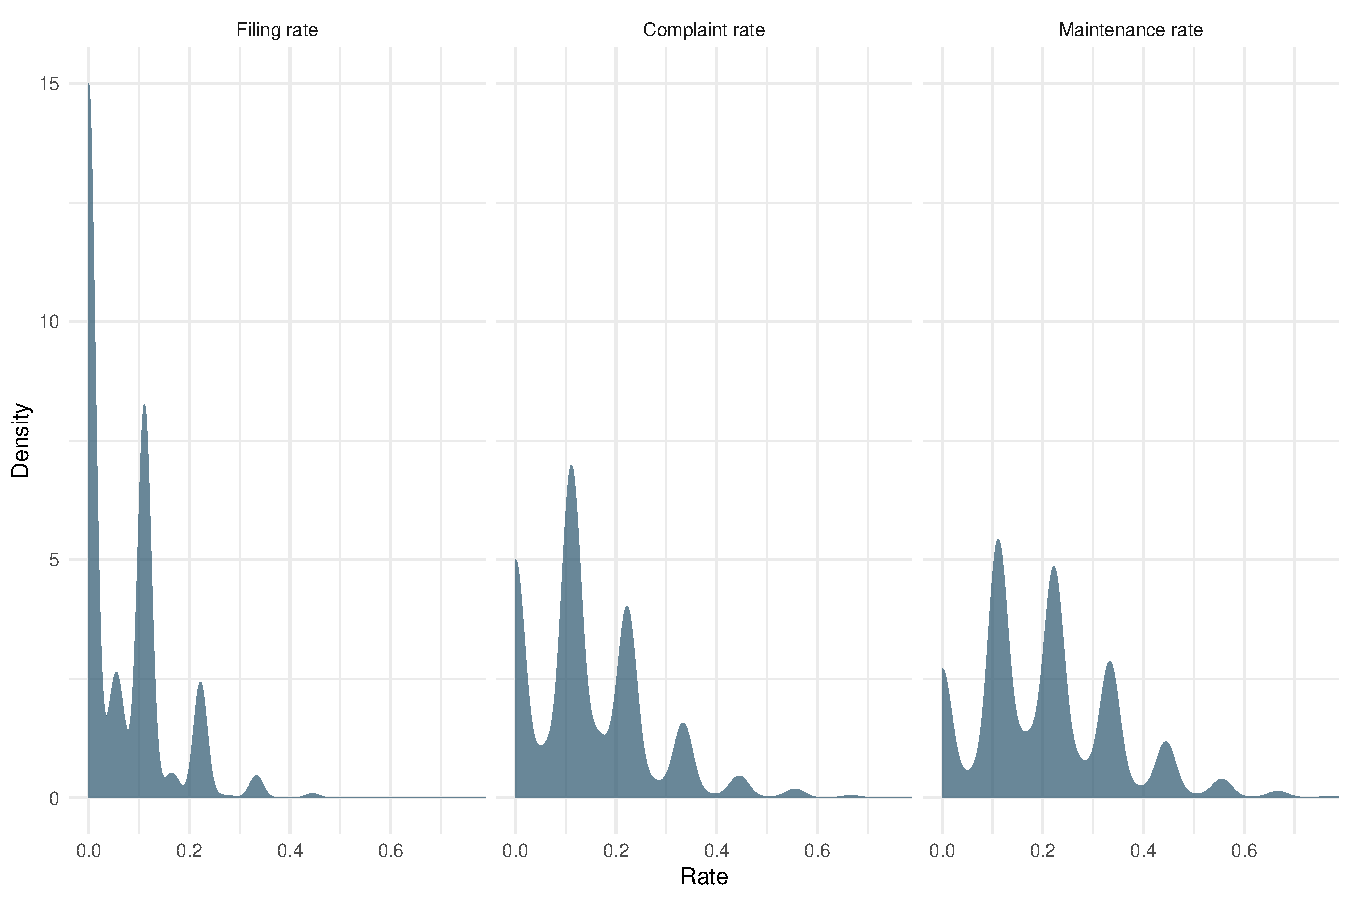
\includegraphics[width=0.95\linewidth,height=\textheight,keepaspectratio]{outer-sorting-baseline_files/figure-pdf/rate-histograms-1.pdf}

}

\caption{Distribution of realized filing, complaint, and maintenance
rates across simulated buildings.}

\end{figure}%

\subsection{Sorting Pattern}\label{sorting-pattern}

\begin{figure}[H]

{\centering 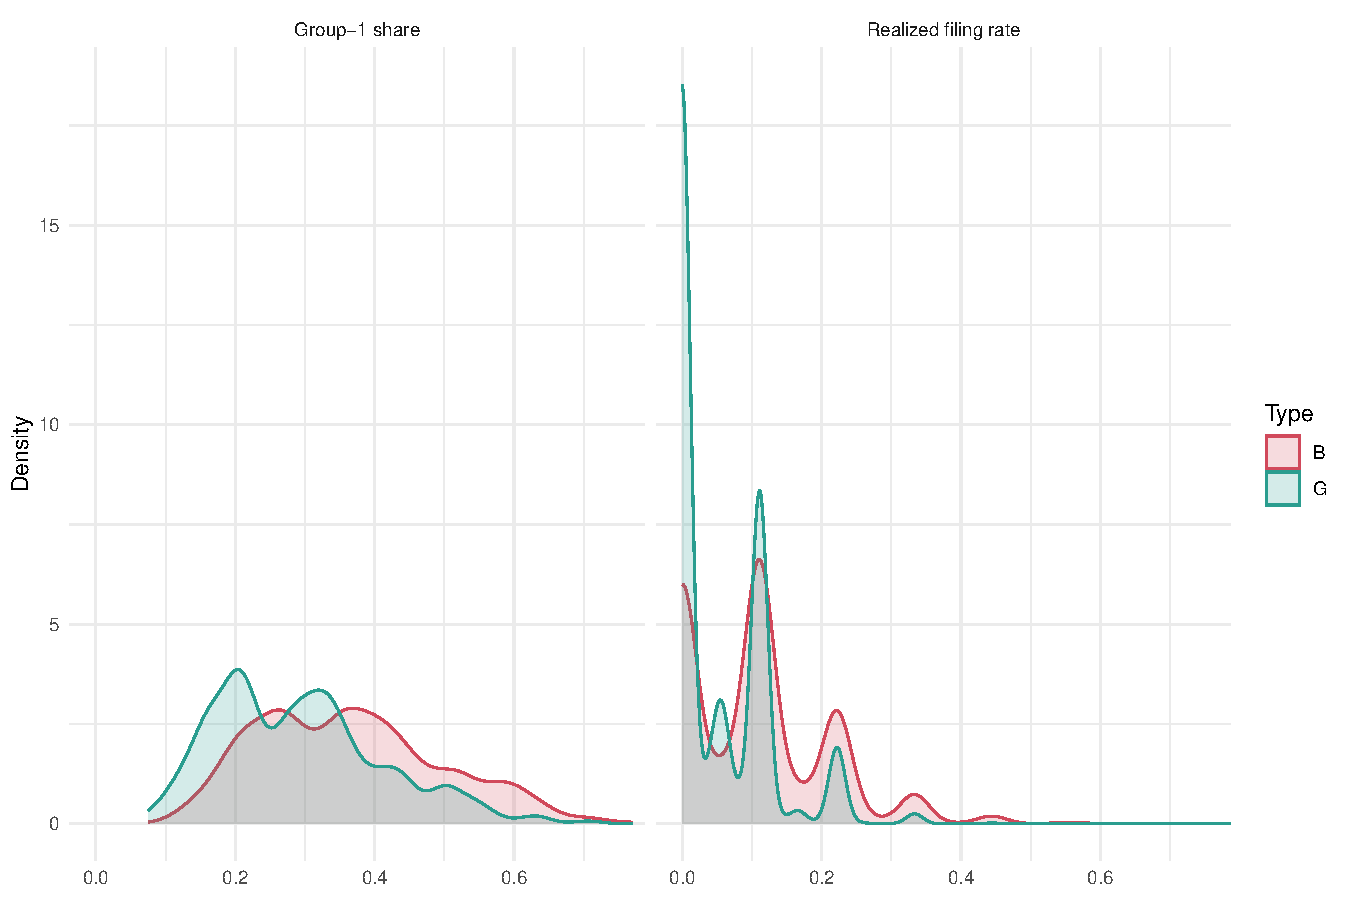
\includegraphics[width=0.92\linewidth,height=\textheight,keepaspectratio]{outer-sorting-baseline_files/figure-pdf/sorting-figure-1.pdf}

}

\caption{Distribution of equilibrium composition shares and realized
filing rates by landlord type.}

\end{figure}%

\subsection{Neighborhood Patterns}\label{neighborhood-patterns}

\begin{table}

\caption{Empirical vs simulated neighborhood distribution summary}
\centering
\begin{tabular}[t]{llrrr}
\toprule
sample & metric & mean & p50 & p90\\
\midrule
Empirical neighborhoods & Neighborhood mean filing rate & 0.0461 & 0.0431 & 0.0855\\
Empirical neighborhoods & Neighborhood mean poverty share & 0.2670 & 0.2525 & 0.4862\\
Simulated neighborhoods & Neighborhood mean filing rate & 0.0648 & 0.0597 & 0.1336\\
Simulated neighborhoods & Neighborhood mean poverty share & 0.3017 & 0.2965 & 0.3240\\
\bottomrule
\end{tabular}
\end{table}

\begin{figure}[H]

{\centering 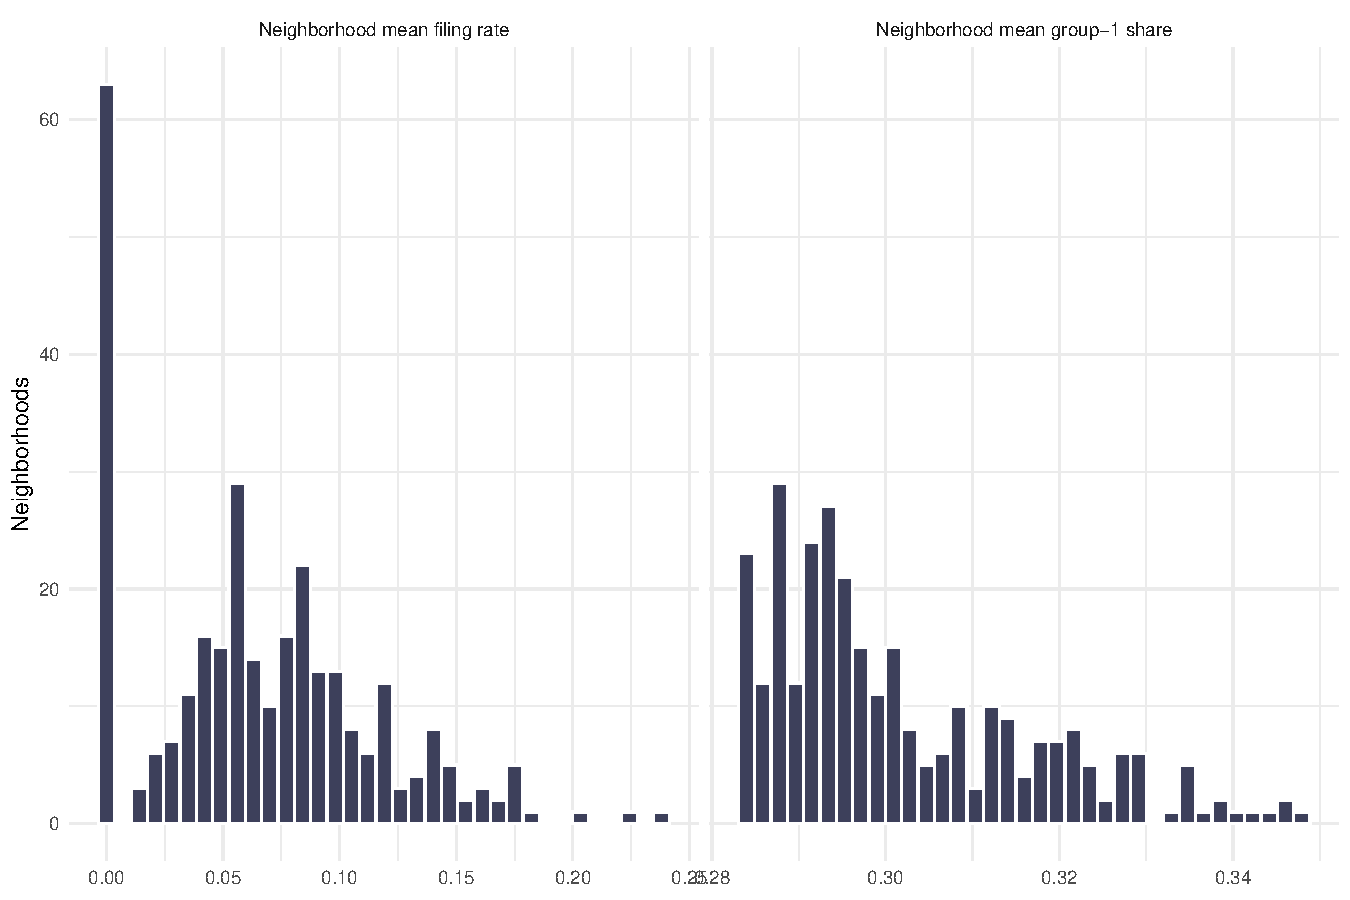
\includegraphics[width=0.95\linewidth,height=\textheight,keepaspectratio]{outer-sorting-baseline_files/figure-pdf/nhood-figures-1.pdf}

}

\caption{Neighborhood-level equilibrium variation in filing rates and
group-1 share, using unit-weighted neighborhood means.}

\end{figure}%

\begin{figure}[H]

{\centering 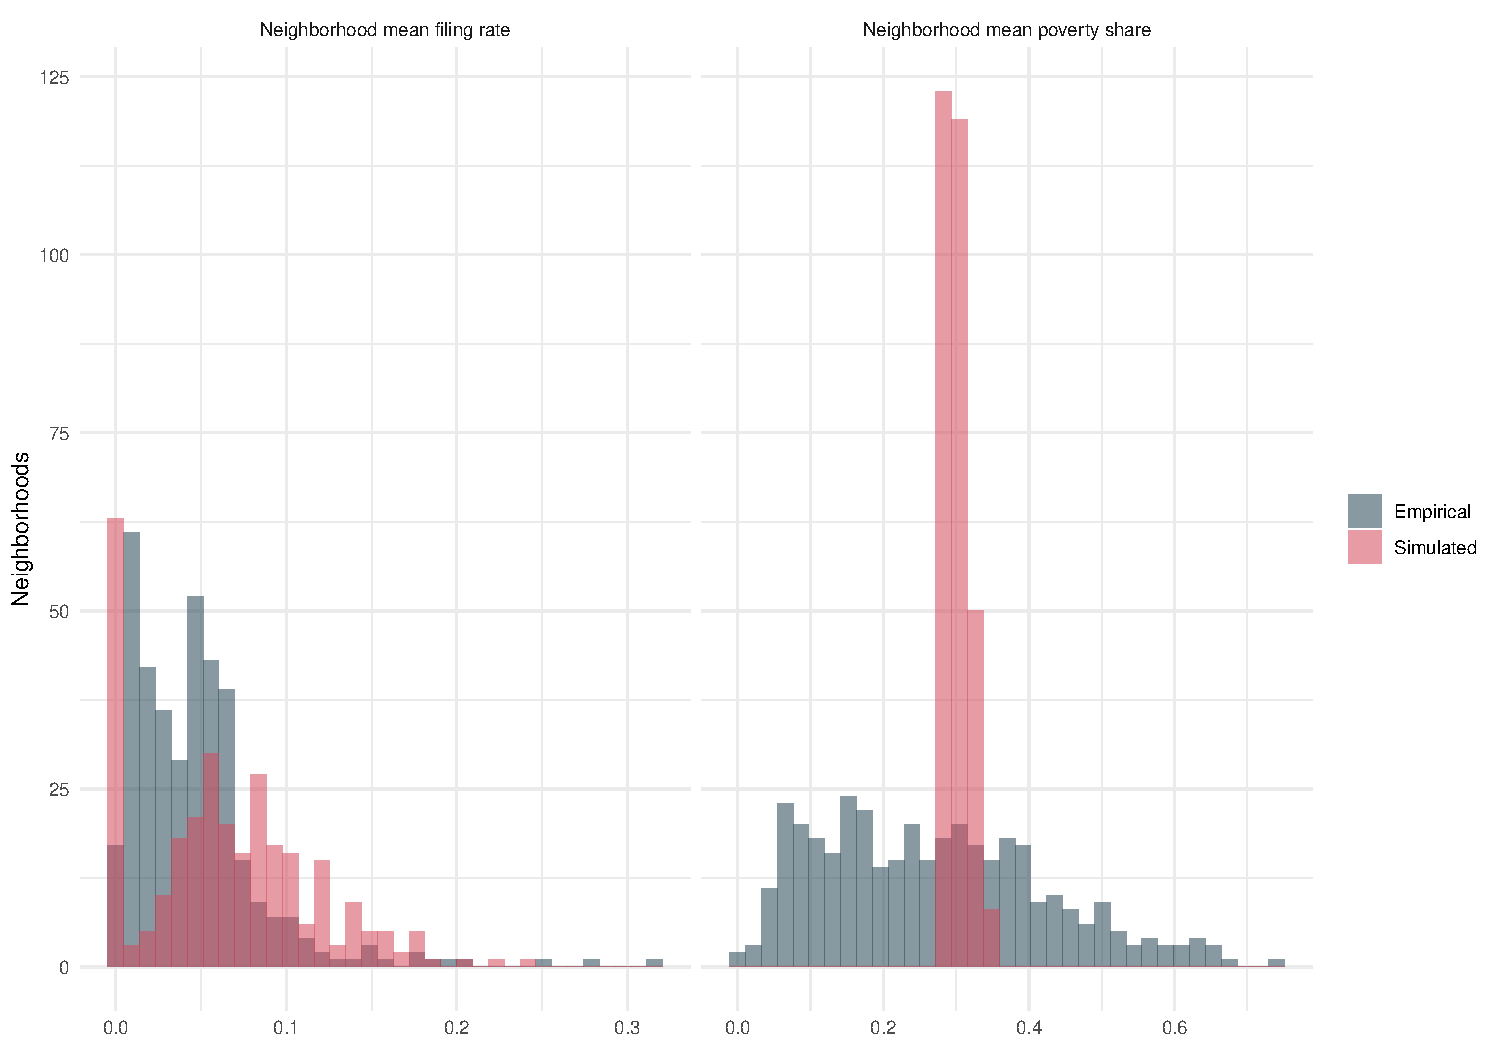
\includegraphics[width=0.95\linewidth,height=\textheight,keepaspectratio]{outer-sorting-baseline_files/figure-pdf/nhood-empirical-vs-sim-1.pdf}

}

\caption{Empirical vs simulated neighborhood distributions for
unit-weighted neighborhood mean filing rates and neighborhood mean
poverty shares.}

\end{figure}%

\begin{figure}[H]

{\centering 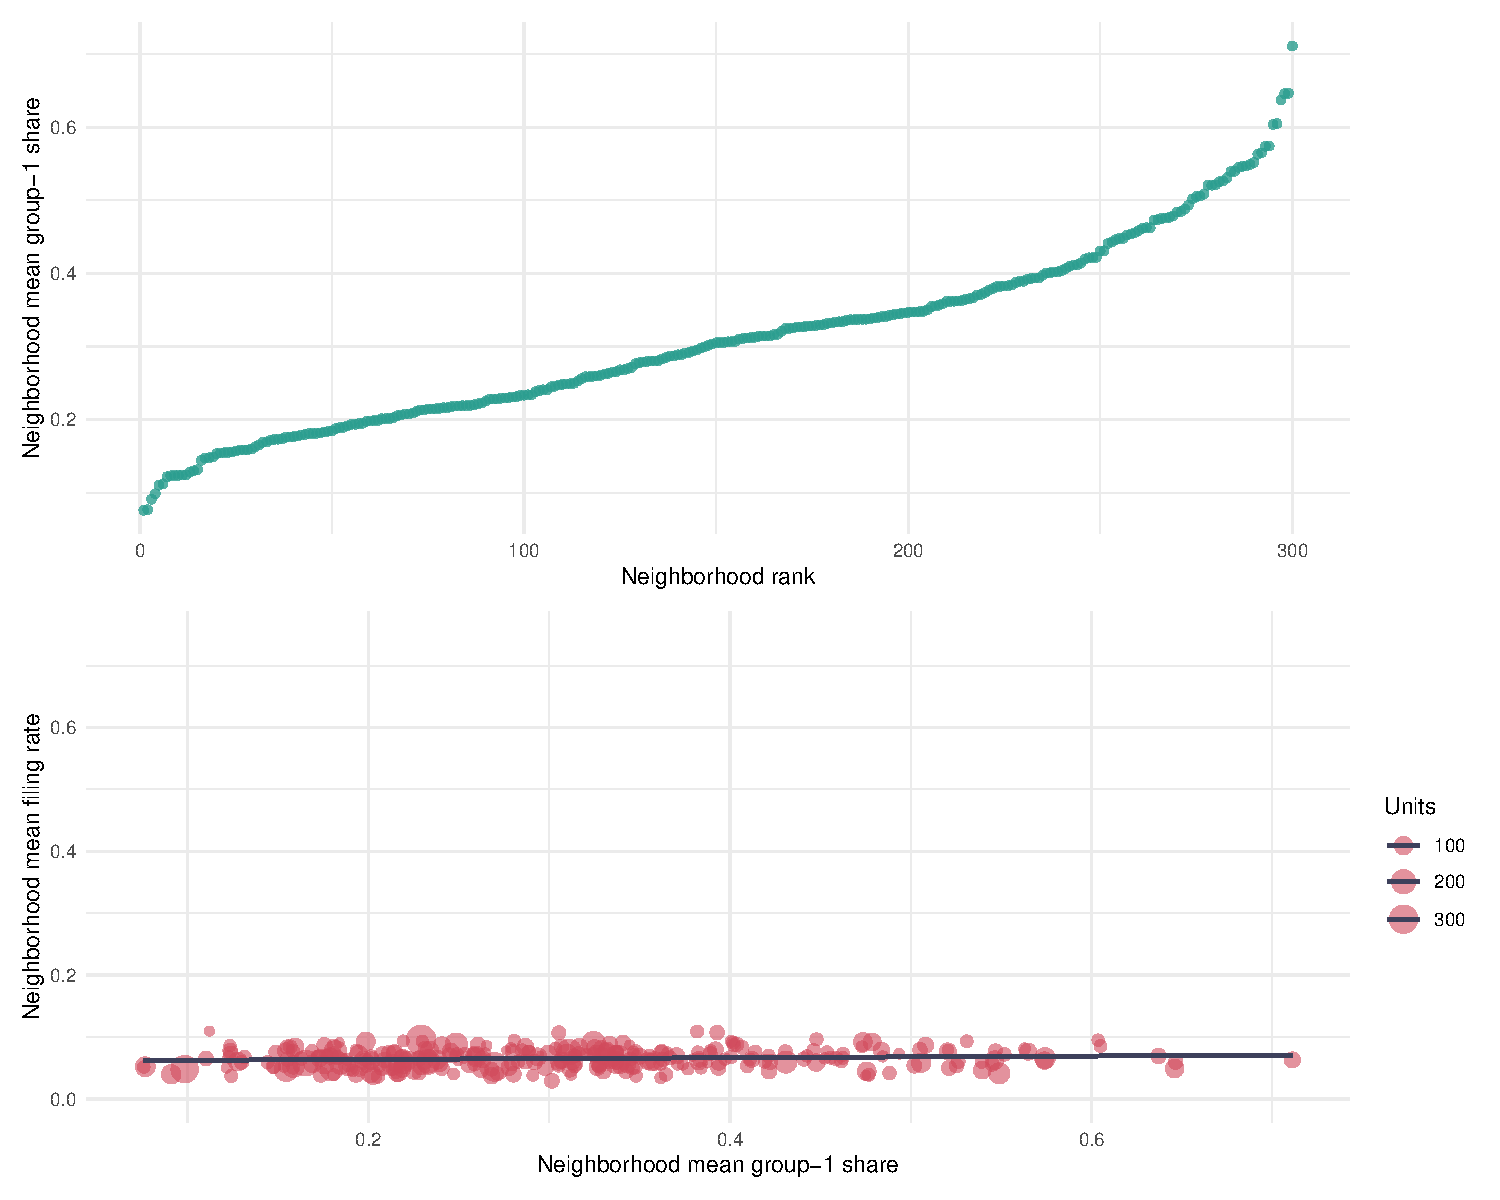
\includegraphics[width=0.95\linewidth,height=\textheight,keepaspectratio]{outer-sorting-baseline_files/figure-pdf/nhood-diagnostics-1.pdf}

}

\caption{Neighborhood diagnostic views: ranked neighborhood group-1
shares and neighborhood mean filing rates against neighborhood mean
group-1 shares.}

\end{figure}%

\begin{figure}[H]

{\centering 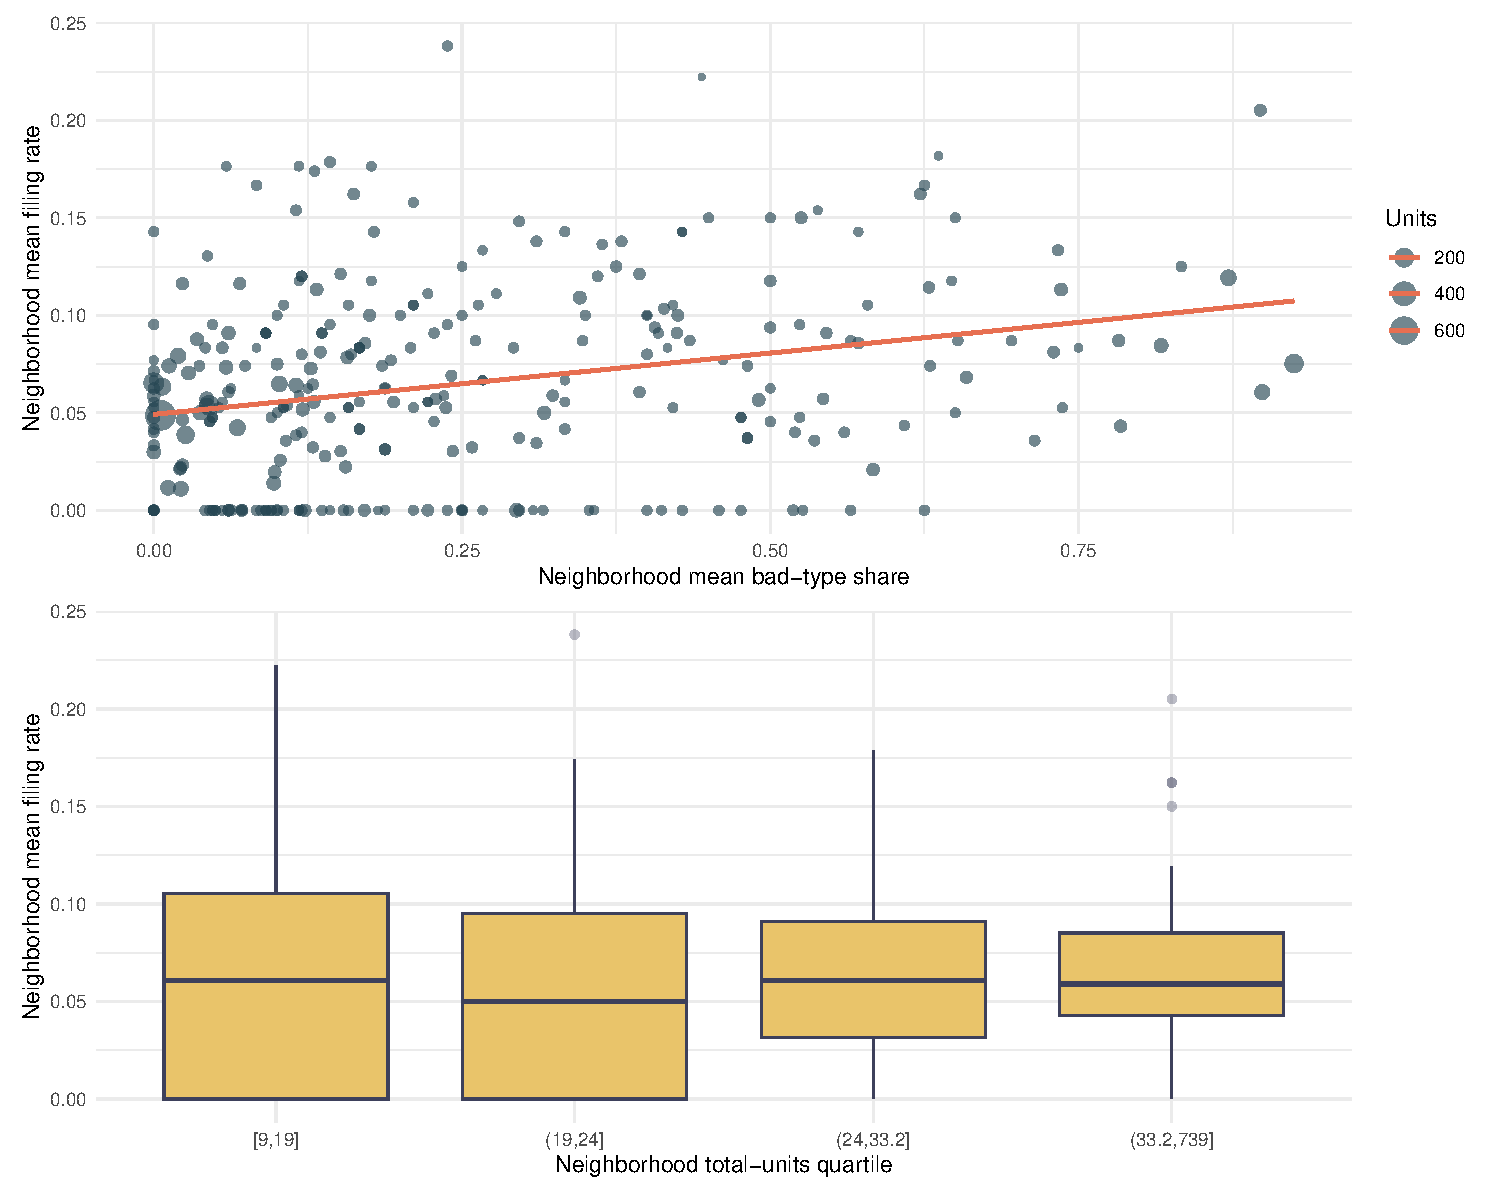
\includegraphics[width=0.95\linewidth,height=\textheight,keepaspectratio]{outer-sorting-baseline_files/figure-pdf/nhood-filing-drivers-1.pdf}

}

\caption{Neighborhood filing-rate variation against neighborhood
bad-type share and by neighborhood size.}

\end{figure}%

\section{First-Pass Calibration
Targets}\label{first-pass-calibration-targets}

The first-pass calibration objective uses a compact 12-moment target
set:

\begin{enumerate}
\def\labelenumi{\arabic{enumi}.}
\tightlist
\item
  Three marginal means: filing, maintenance, and complaint rates.
\item
  Three zero shares: zero filings, zero maintenance, and zero
  complaints.
\item
  Two sorting moments: composition on high filing within neighborhood,
  and composition for the top filing bin relative to the low filing bin
  within neighborhood.
\item
  Two complaint-gradient moments: complaints on composition, and
  complaints on composition \(\times\) high filing.
\item
  One maintenance-discipline moment: maintenance on complaint intensity.
\item
  One filing-dispersion moment: residual SD of filing rates after
  neighborhood fixed effects.
\end{enumerate}

The current calibration target product is
outer\_sorting\_empirical\_moments, so the moment comparison table below
should be read as an empirical fit diagnostic rather than a
self-calibration check.

\begin{table}

\caption{Calibration target vs simulated moments}
\centering
\begin{tabular}[t]{lrrrr}
\toprule
moment & target & simulated & weight & diff\\
\midrule
mean\_f\_rate & 0.0390 & 0.1669 & 10 & -0.1280\\
mean\_m\_rate & 0.0554 & 0.2082 & 10 & -0.1530\\
mean\_c\_rate & 0.0694 & 0.1366 & 10 & -0.0672\\
zero\_share\_f & 0.7633 & 0.7994 & 5 & -0.0361\\
zero\_share\_m & 0.7409 & 0.7568 & 5 & -0.0159\\
zero\_share\_c & 0.5370 & 0.8246 & 5 & -0.2880\\
sorting\_coef\_high\_filing\_nhood & 0.0048 & 0.0974 & 5 & -0.0926\\
sorting\_coef\_high\_bin\_nhood & 0.0057 & 0.0930 & 5 & -0.0873\\
beta\_ppml\_s & -0.0719 & 0.4595 & 2 & -0.5310\\
beta\_ppml\_s\_x\_high\_filing & 0.0168 & 0.0245 & 2 & -0.0077\\
beta\_maint\_on\_log1p\_c\_rate & 2.8806 & 0.1684 & 2 & 2.7100\\
filing\_resid\_sd\_nhood\_fe & 0.1155 & 0.3694 & 5 & -0.2540\\
\bottomrule
\end{tabular}
\end{table}

\subsection{Current Calibration Run}\label{current-calibration-run}

\begin{table}

\caption{Calibration run summary}
\centering
\begin{tabular}[t]{ll}
\toprule
metric & value\\
\midrule
Target product & outer\_sorting\_empirical\_moments\\
Convergence code & 1\\
Objective & 16.5445\\
Evaluations & 308\\
\bottomrule
\end{tabular}
\end{table}

The current empirical calibration run did not fully converge in the
optimizer. The fixed-point solver inside each simulation evaluation is
behaving, but the outer optimizer stopped at convergence code 1 with
objective 16.545 after 308 evaluations.

\begin{table}

\caption{Baseline vs calibrated parameters}
\centering
\begin{tabular}[t]{lrrr}
\toprule
parameter & baseline & calibrated & change\\
\midrule
p\_bad\_shape1 & 2.00 & 2.1615 & 0.1615\\
p\_bad\_shape2 & 6.00 & 6.2056 & 0.2056\\
Dalph & 6.00 & 10.1412 & 4.1412\\
aM & -1.70 & -1.5930 & 0.1070\\
bM\_theta & -0.20 & -0.0498 & 0.1502\\
bM\_C & 0.12 & 0.3364 & 0.2164\\
aC & -2.10 & -1.9986 & 0.1014\\
bC\_theta & 0.35 & 0.2616 & -0.0884\\
bC\_s & 0.35 & 0.0931 & -0.2569\\
bC\_M & -0.10 & -0.2733 & -0.1733\\
aF & -3.00 & -2.1685 & 0.8315\\
bF\_theta & 0.70 & 0.8878 & 0.1878\\
bF\_delta & 1.10 & 1.3379 & 0.2379\\
\bottomrule
\end{tabular}
\end{table}

\begin{table}

\caption{Largest calibration moment misses}
\centering
\begin{tabular}[t]{lrrrr}
\toprule
moment & target & simulated & diff & weighted\_sq\_error\\
\midrule
beta\_maint\_on\_log1p\_c\_rate & 2.8806 & 0.1684 & 2.7123 & 14.7126\\
beta\_ppml\_s & -0.0719 & 0.4595 & -0.5314 & 0.5648\\
zero\_share\_c & 0.5370 & 0.8246 & -0.2876 & 0.4136\\
filing\_resid\_sd\_nhood\_fe & 0.1155 & 0.3694 & -0.2539 & 0.3224\\
mean\_m\_rate & 0.0554 & 0.2082 & -0.1528 & 0.2335\\
mean\_f\_rate & 0.0390 & 0.1669 & -0.1279 & 0.1636\\
mean\_c\_rate & 0.0694 & 0.1366 & -0.0672 & 0.0451\\
sorting\_coef\_high\_filing\_nhood & 0.0048 & 0.0974 & -0.0926 & 0.0429\\
\bottomrule
\end{tabular}
\end{table}

The largest misses are informative. In the current run, the model still
overpredicts filing and maintenance rates, produces too little zero
mass, and generates much stronger sorting gradients than the empirical
target. The maintenance-discipline moment is also much smaller in the
simulated equilibrium than in the data target.

\section{Current Interpretation}\label{current-interpretation}

The baseline equilibrium does the basic qualitative work the model is
supposed to do: bad-type buildings end up with higher filing rates and
higher group-1 shares, while maintenance is lower on average in those
buildings and complaints are higher. The citywide mass constraint is
satisfied tightly and the deterministic fixed point converges quickly.

The empirical calibration results suggest that the current baseline is
directionally coherent but still too aggressive relative to the data.
The main gaps are in outcome levels, zero mass, sorting strength, and
the complaint-maintenance discipline link.

The next substantive question is whether these misses come mostly from
the empirical target construction, from the poverty-share proxy for
composition, or from the structural tightness of the filing, complaint,
and maintenance blocks themselves.




\end{document}
